\section{The K-mer Representation Quality} \label{sec:K_mer_Representation}

\blindtext

% \begin{figure}[!hbt]
%     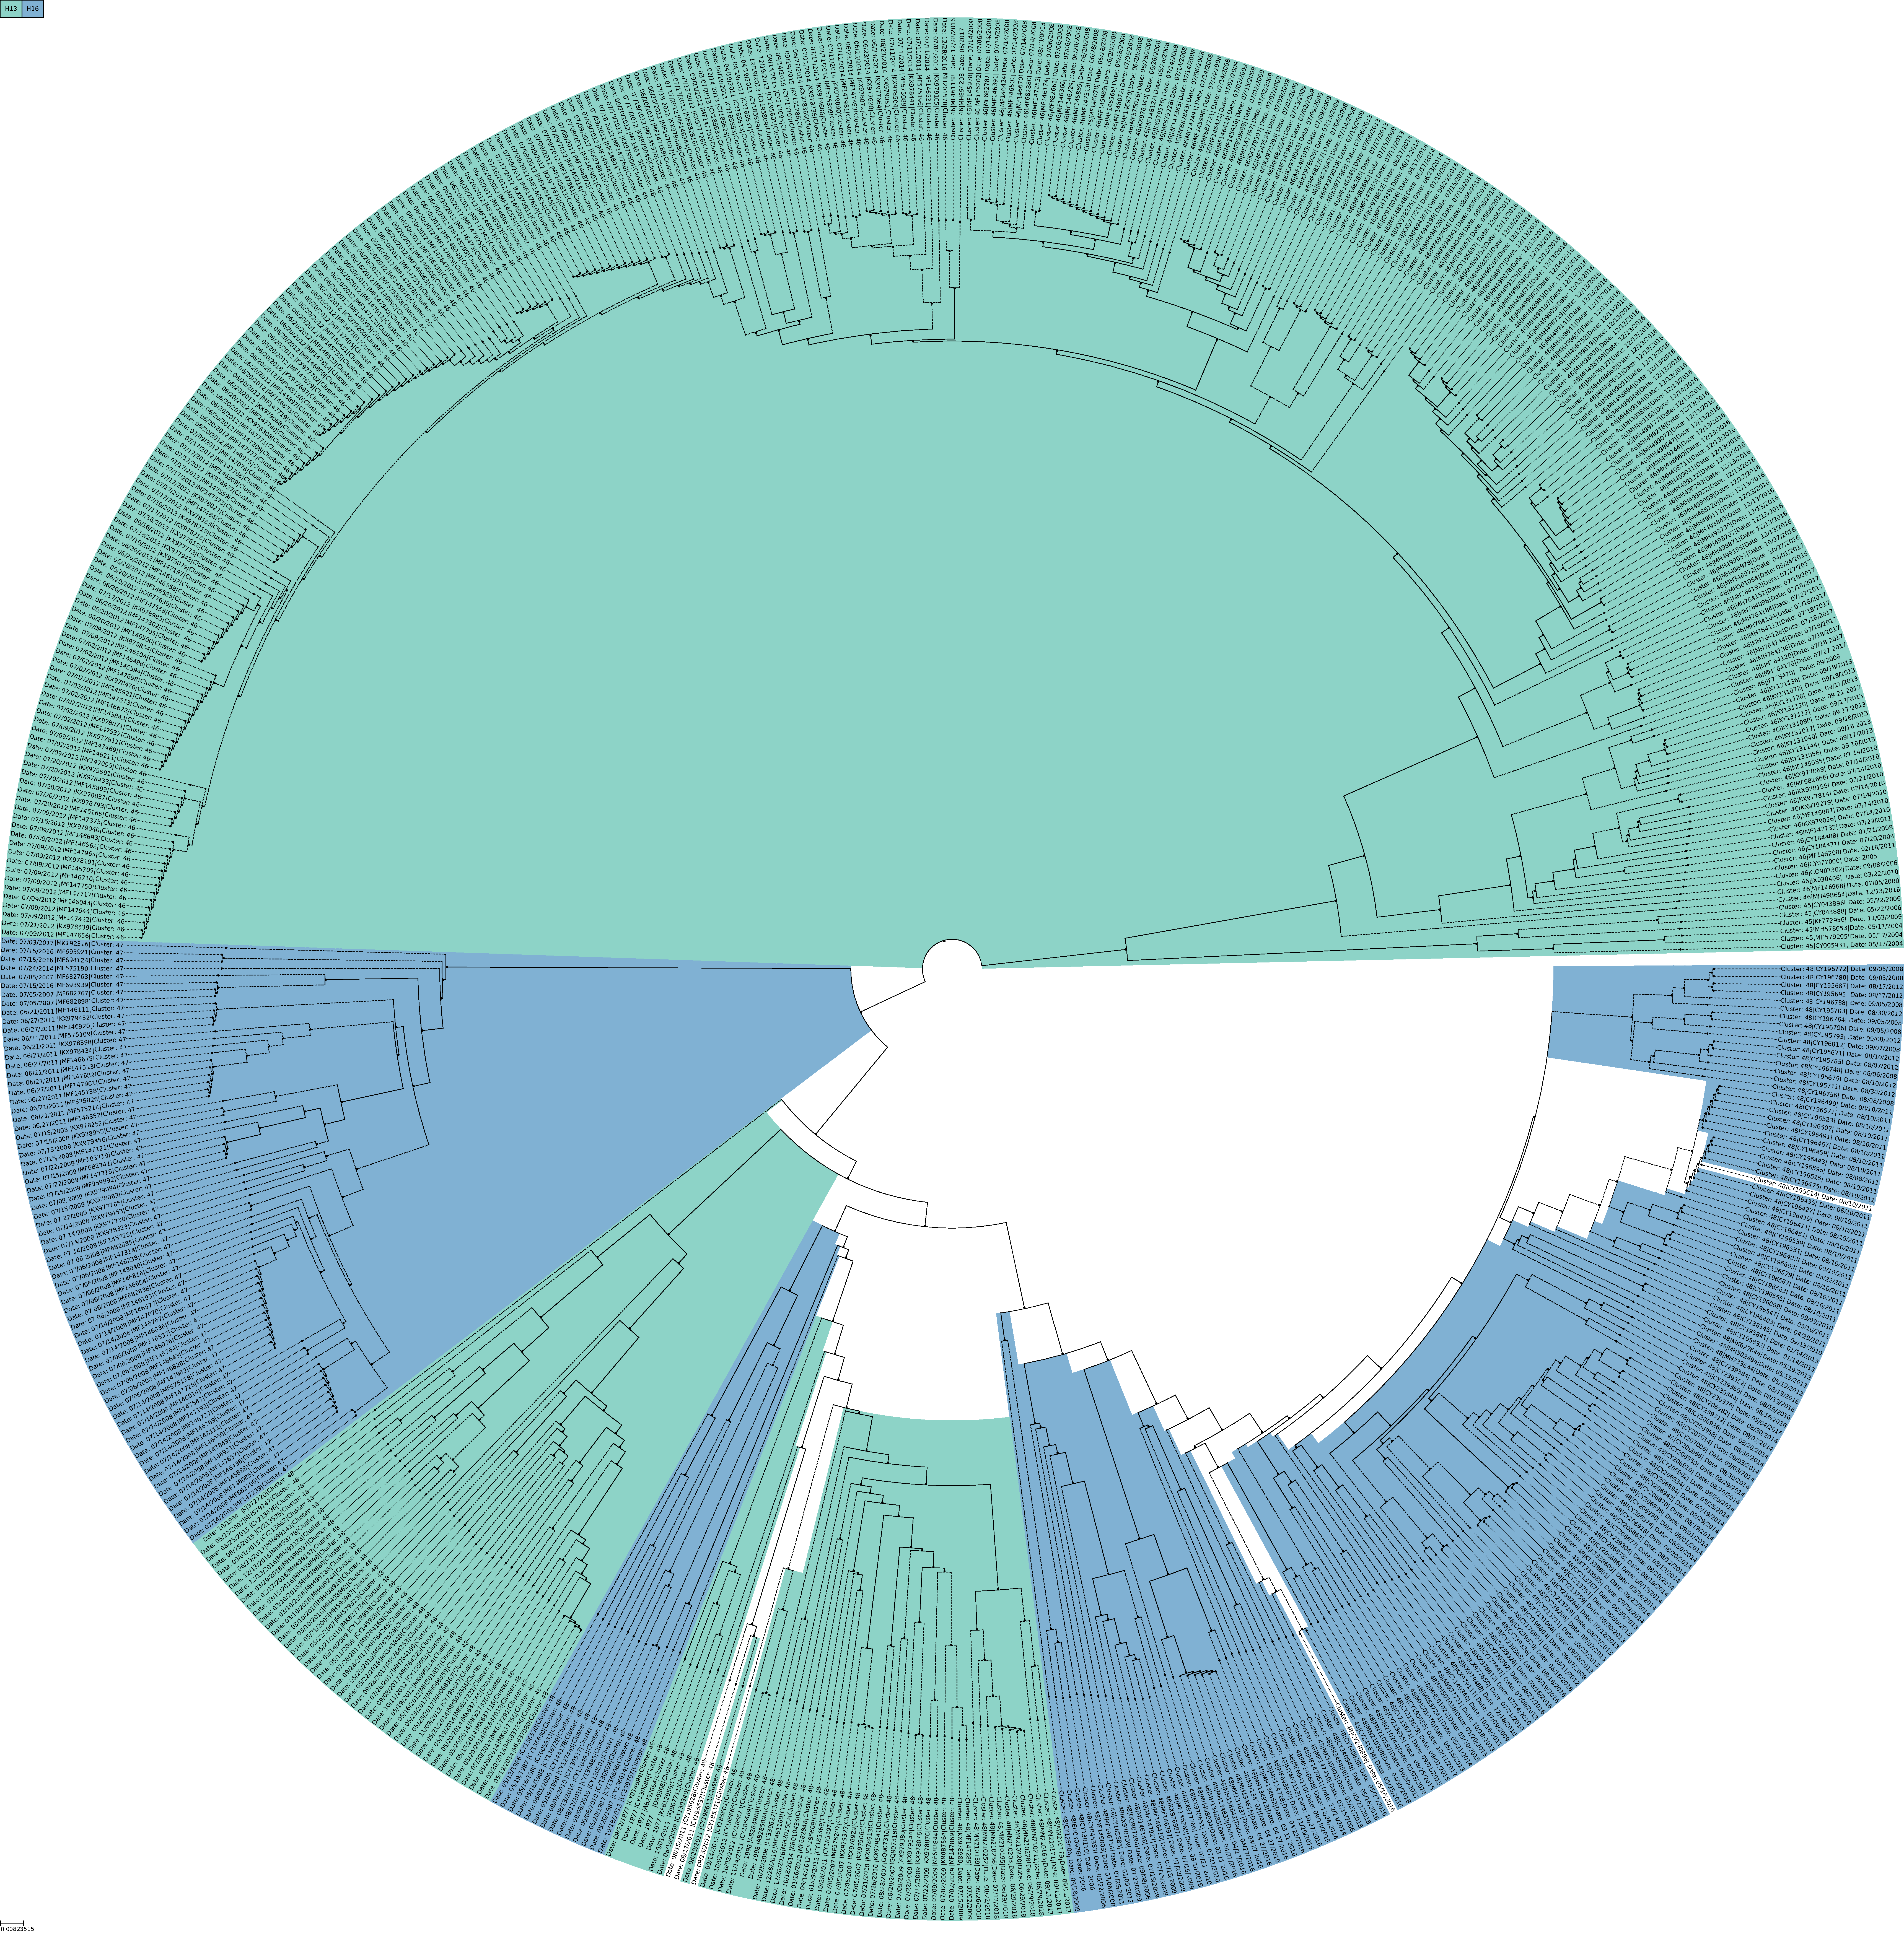
\includegraphics[width=\dimexpr\textwidth-2\fboxsep-2\fboxrule,fbox]{PCA/Clustertree_Segment_4_H_Knee_Zoom.pdf}
%     \caption[H13/H16 Simple Clustering Example with \Acrshort{PCA}]{\textbf{H13/H16 Simple Clustering Example with \Acrshort{PCA}.} .}
%     \label{fig:PCA_Clusteree_Knee_Zoom}
% \end{figure}

% \begin{figure}[!hbt]
%     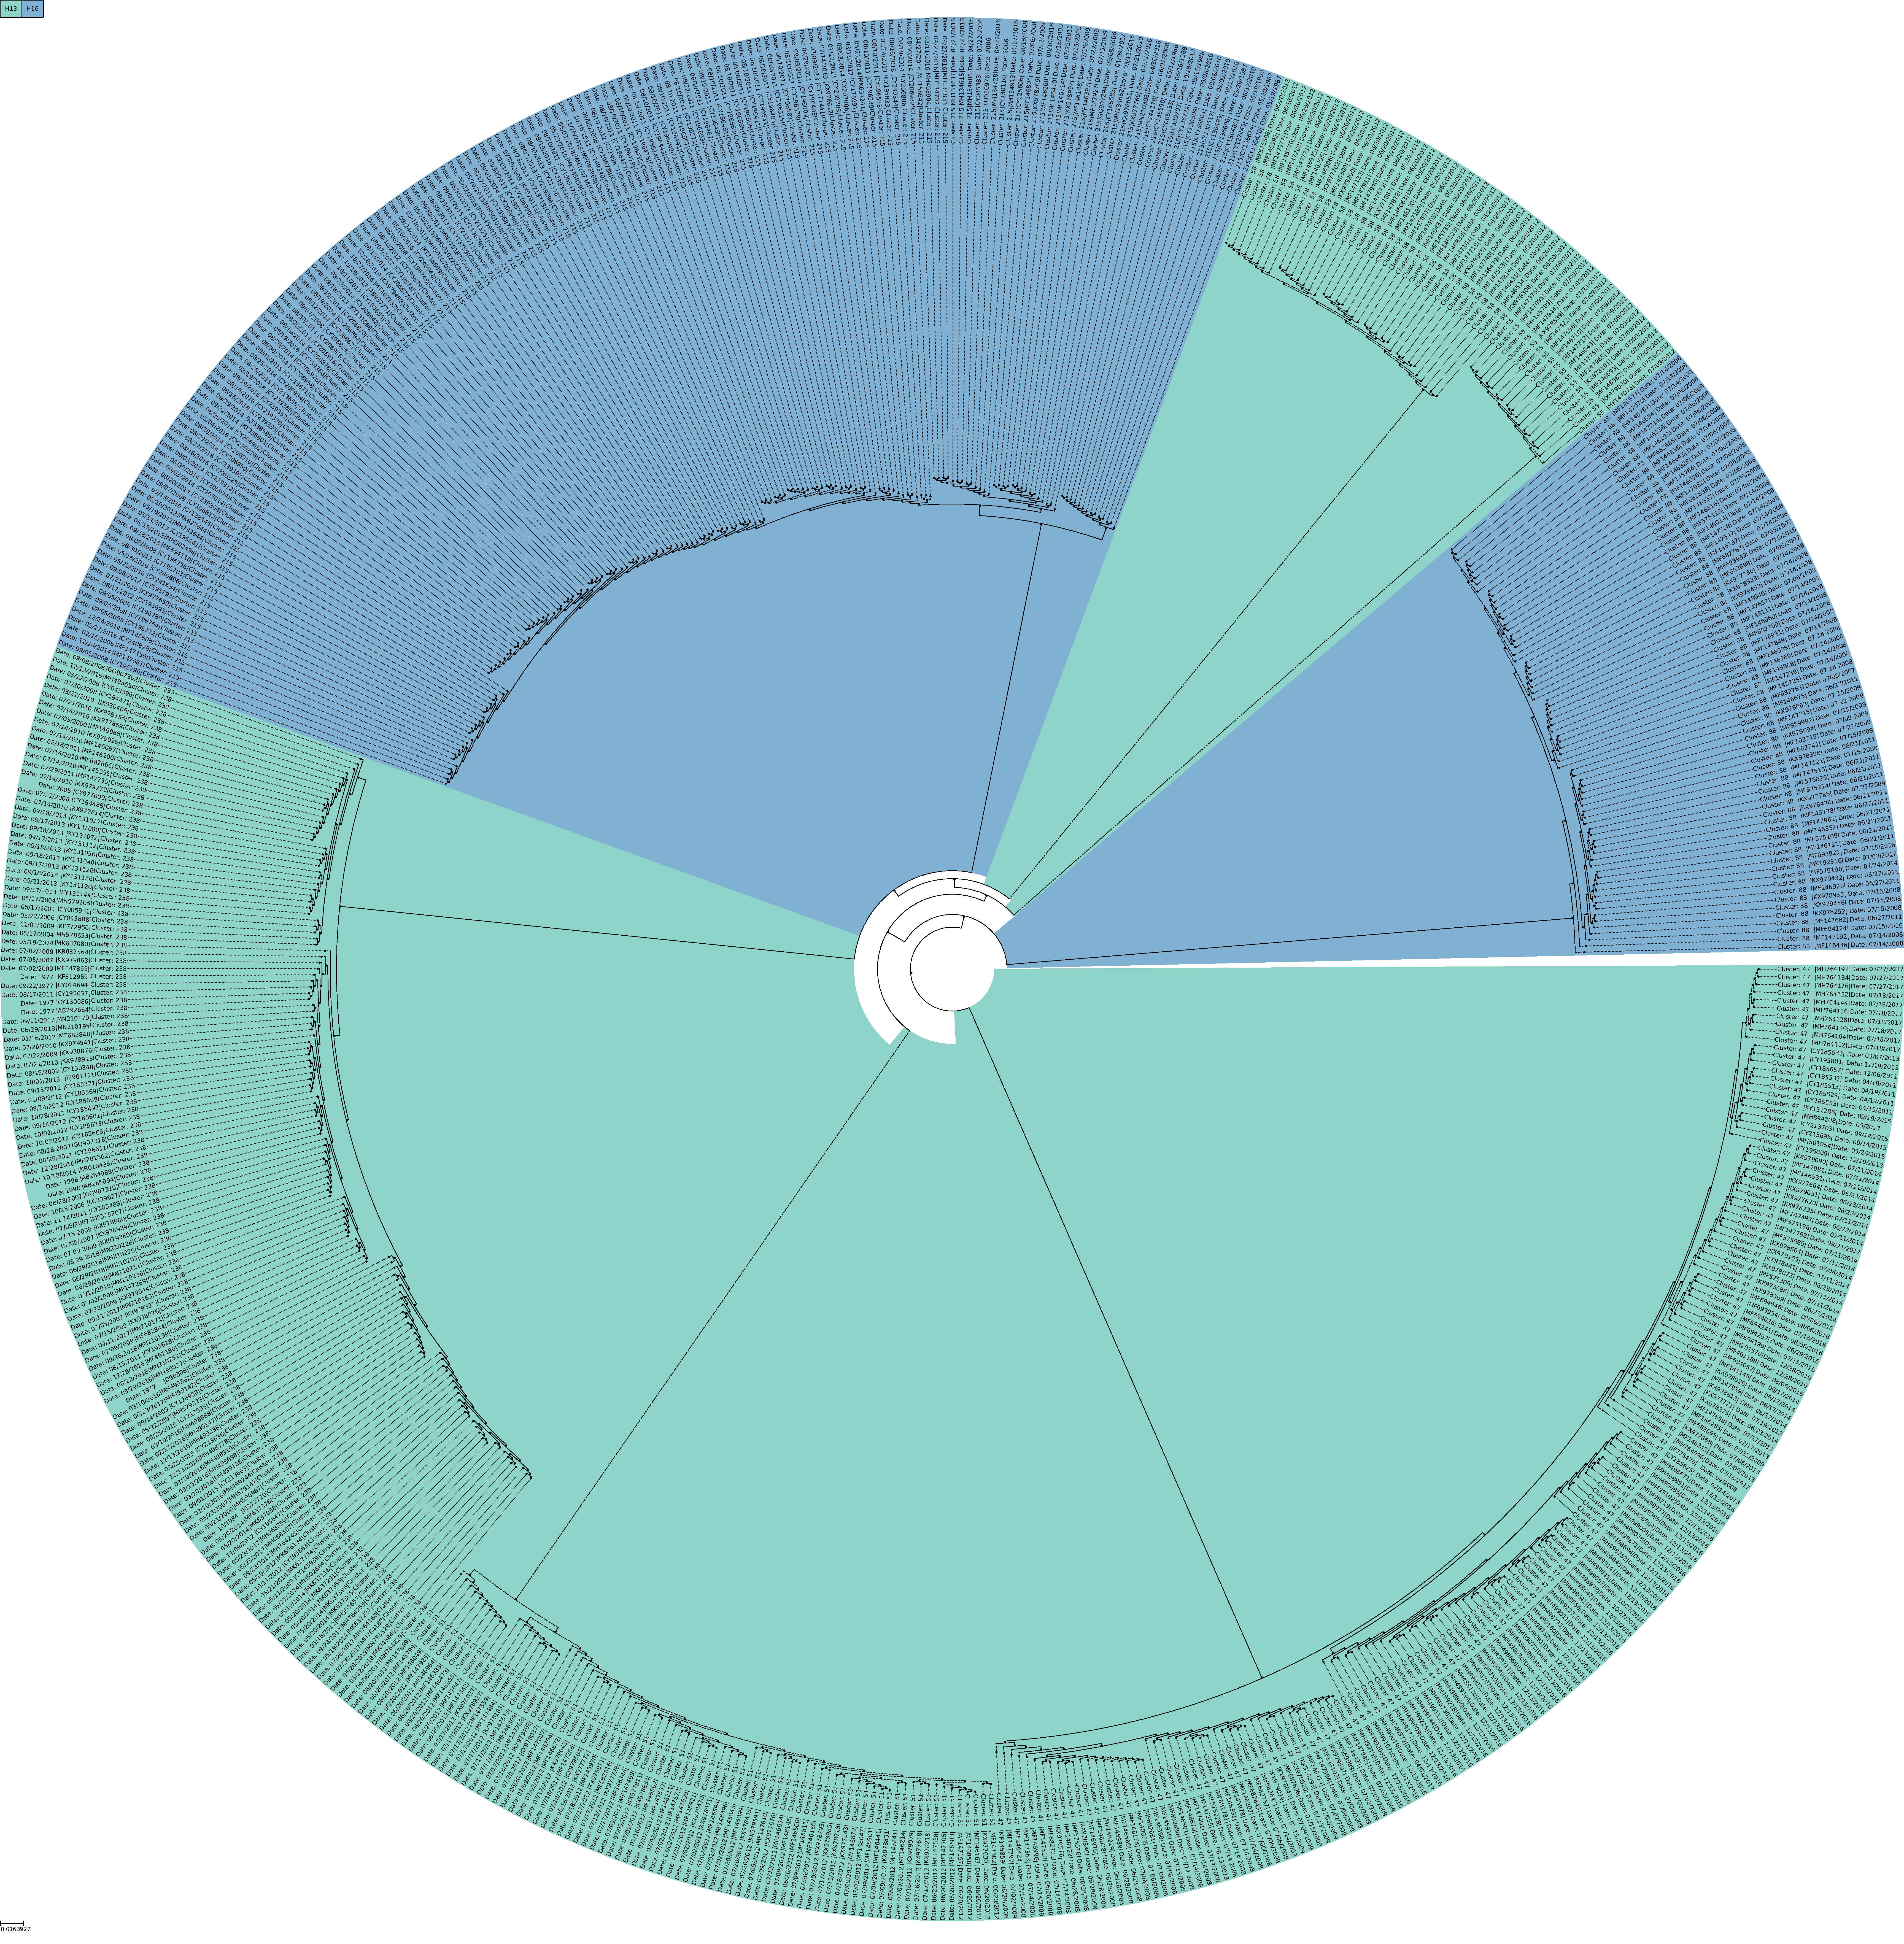
\includegraphics[width=\dimexpr\textwidth-2\fboxsep-2\fboxrule,fbox]{UMAP/Clustertree_Segment_4_H_Knee_Zoom.pdf}
%     \caption[H13/H16 Simple Clustering Example with \Acrshort{UMAP}]{\textbf{H13/H16 Simple Clustering Example with \Acrshort{UMAP}.} .}
%     \label{fig:UMAP_Clusteree_Knee_Zoom}
% \end{figure}

% \begin{figure}[!hbt]
%     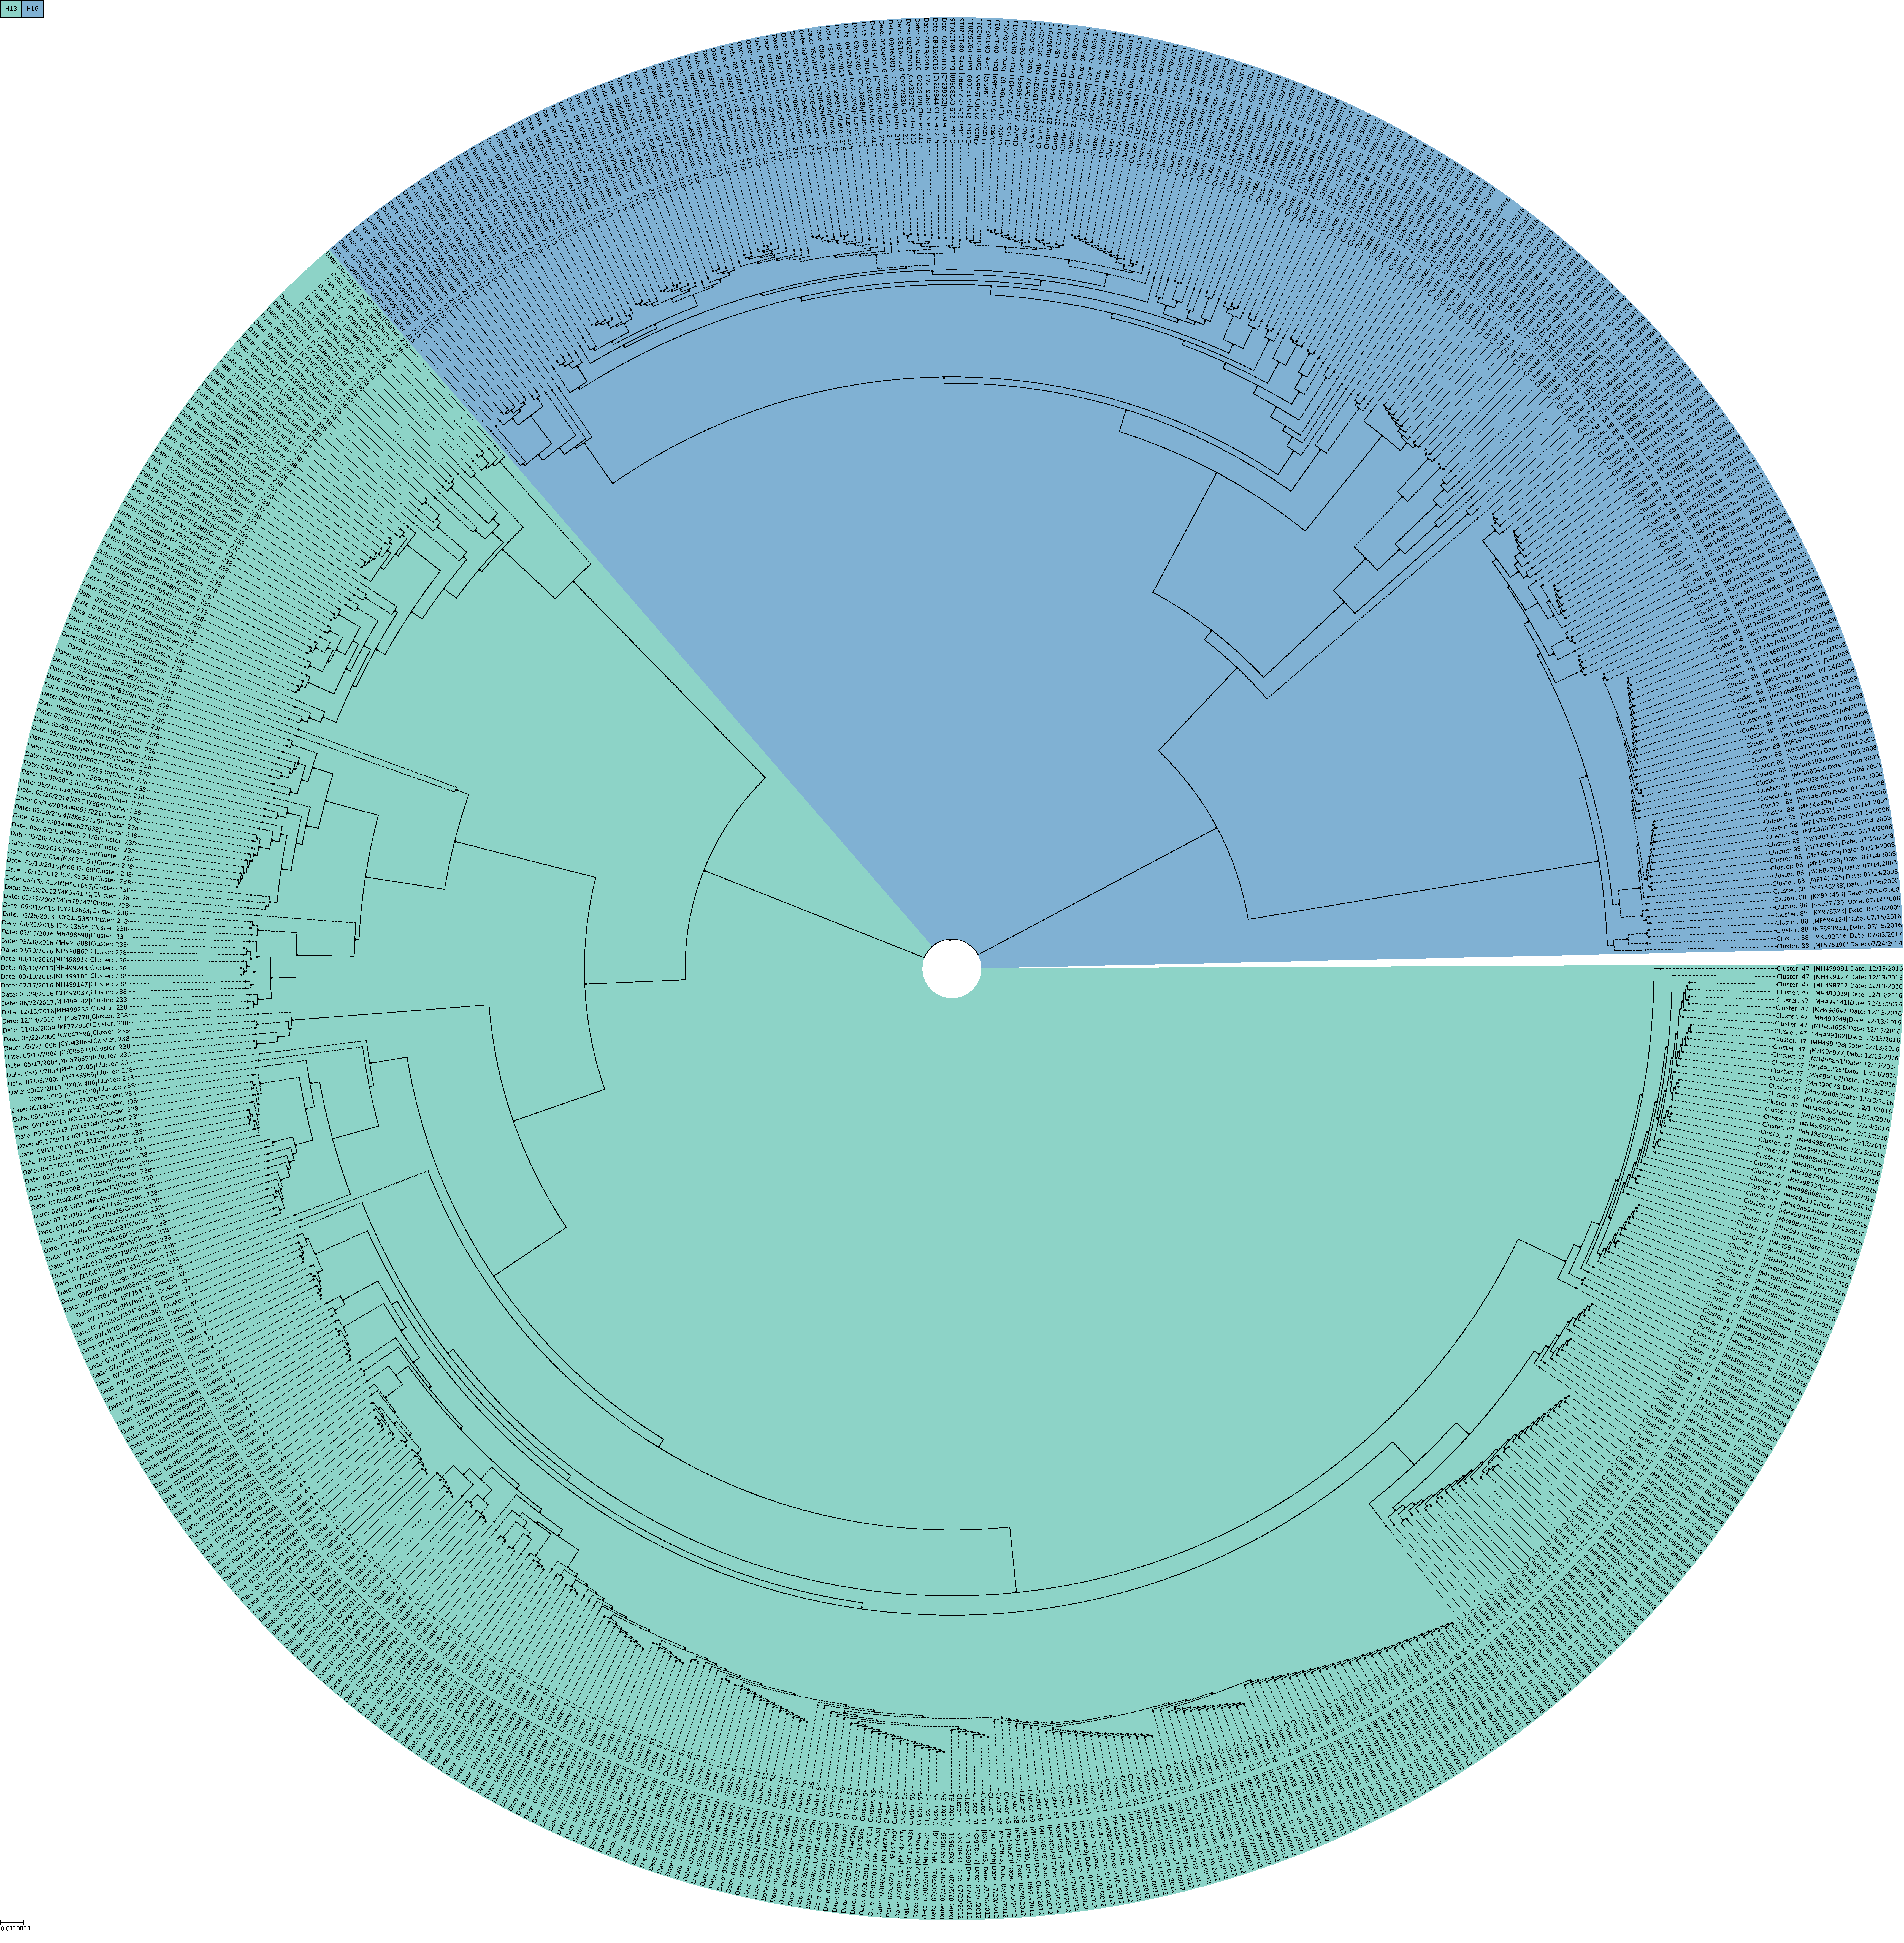
\includegraphics[width=\dimexpr\textwidth-2\fboxsep-2\fboxrule,fbox]{UMAP/Guidetree_Segment_4_H_Focus.pdf}
%     \caption[H13/H16 Simple Clustering Example with \Acrshort{MSA}]{\textbf{H13/H16 Simple Clustering Example with \Acrshort{MSA}.} .}
%     \label{fig:Guidetree_Focus}
% \end{figure}

\begin{figure}[!hbt]
    \centering
    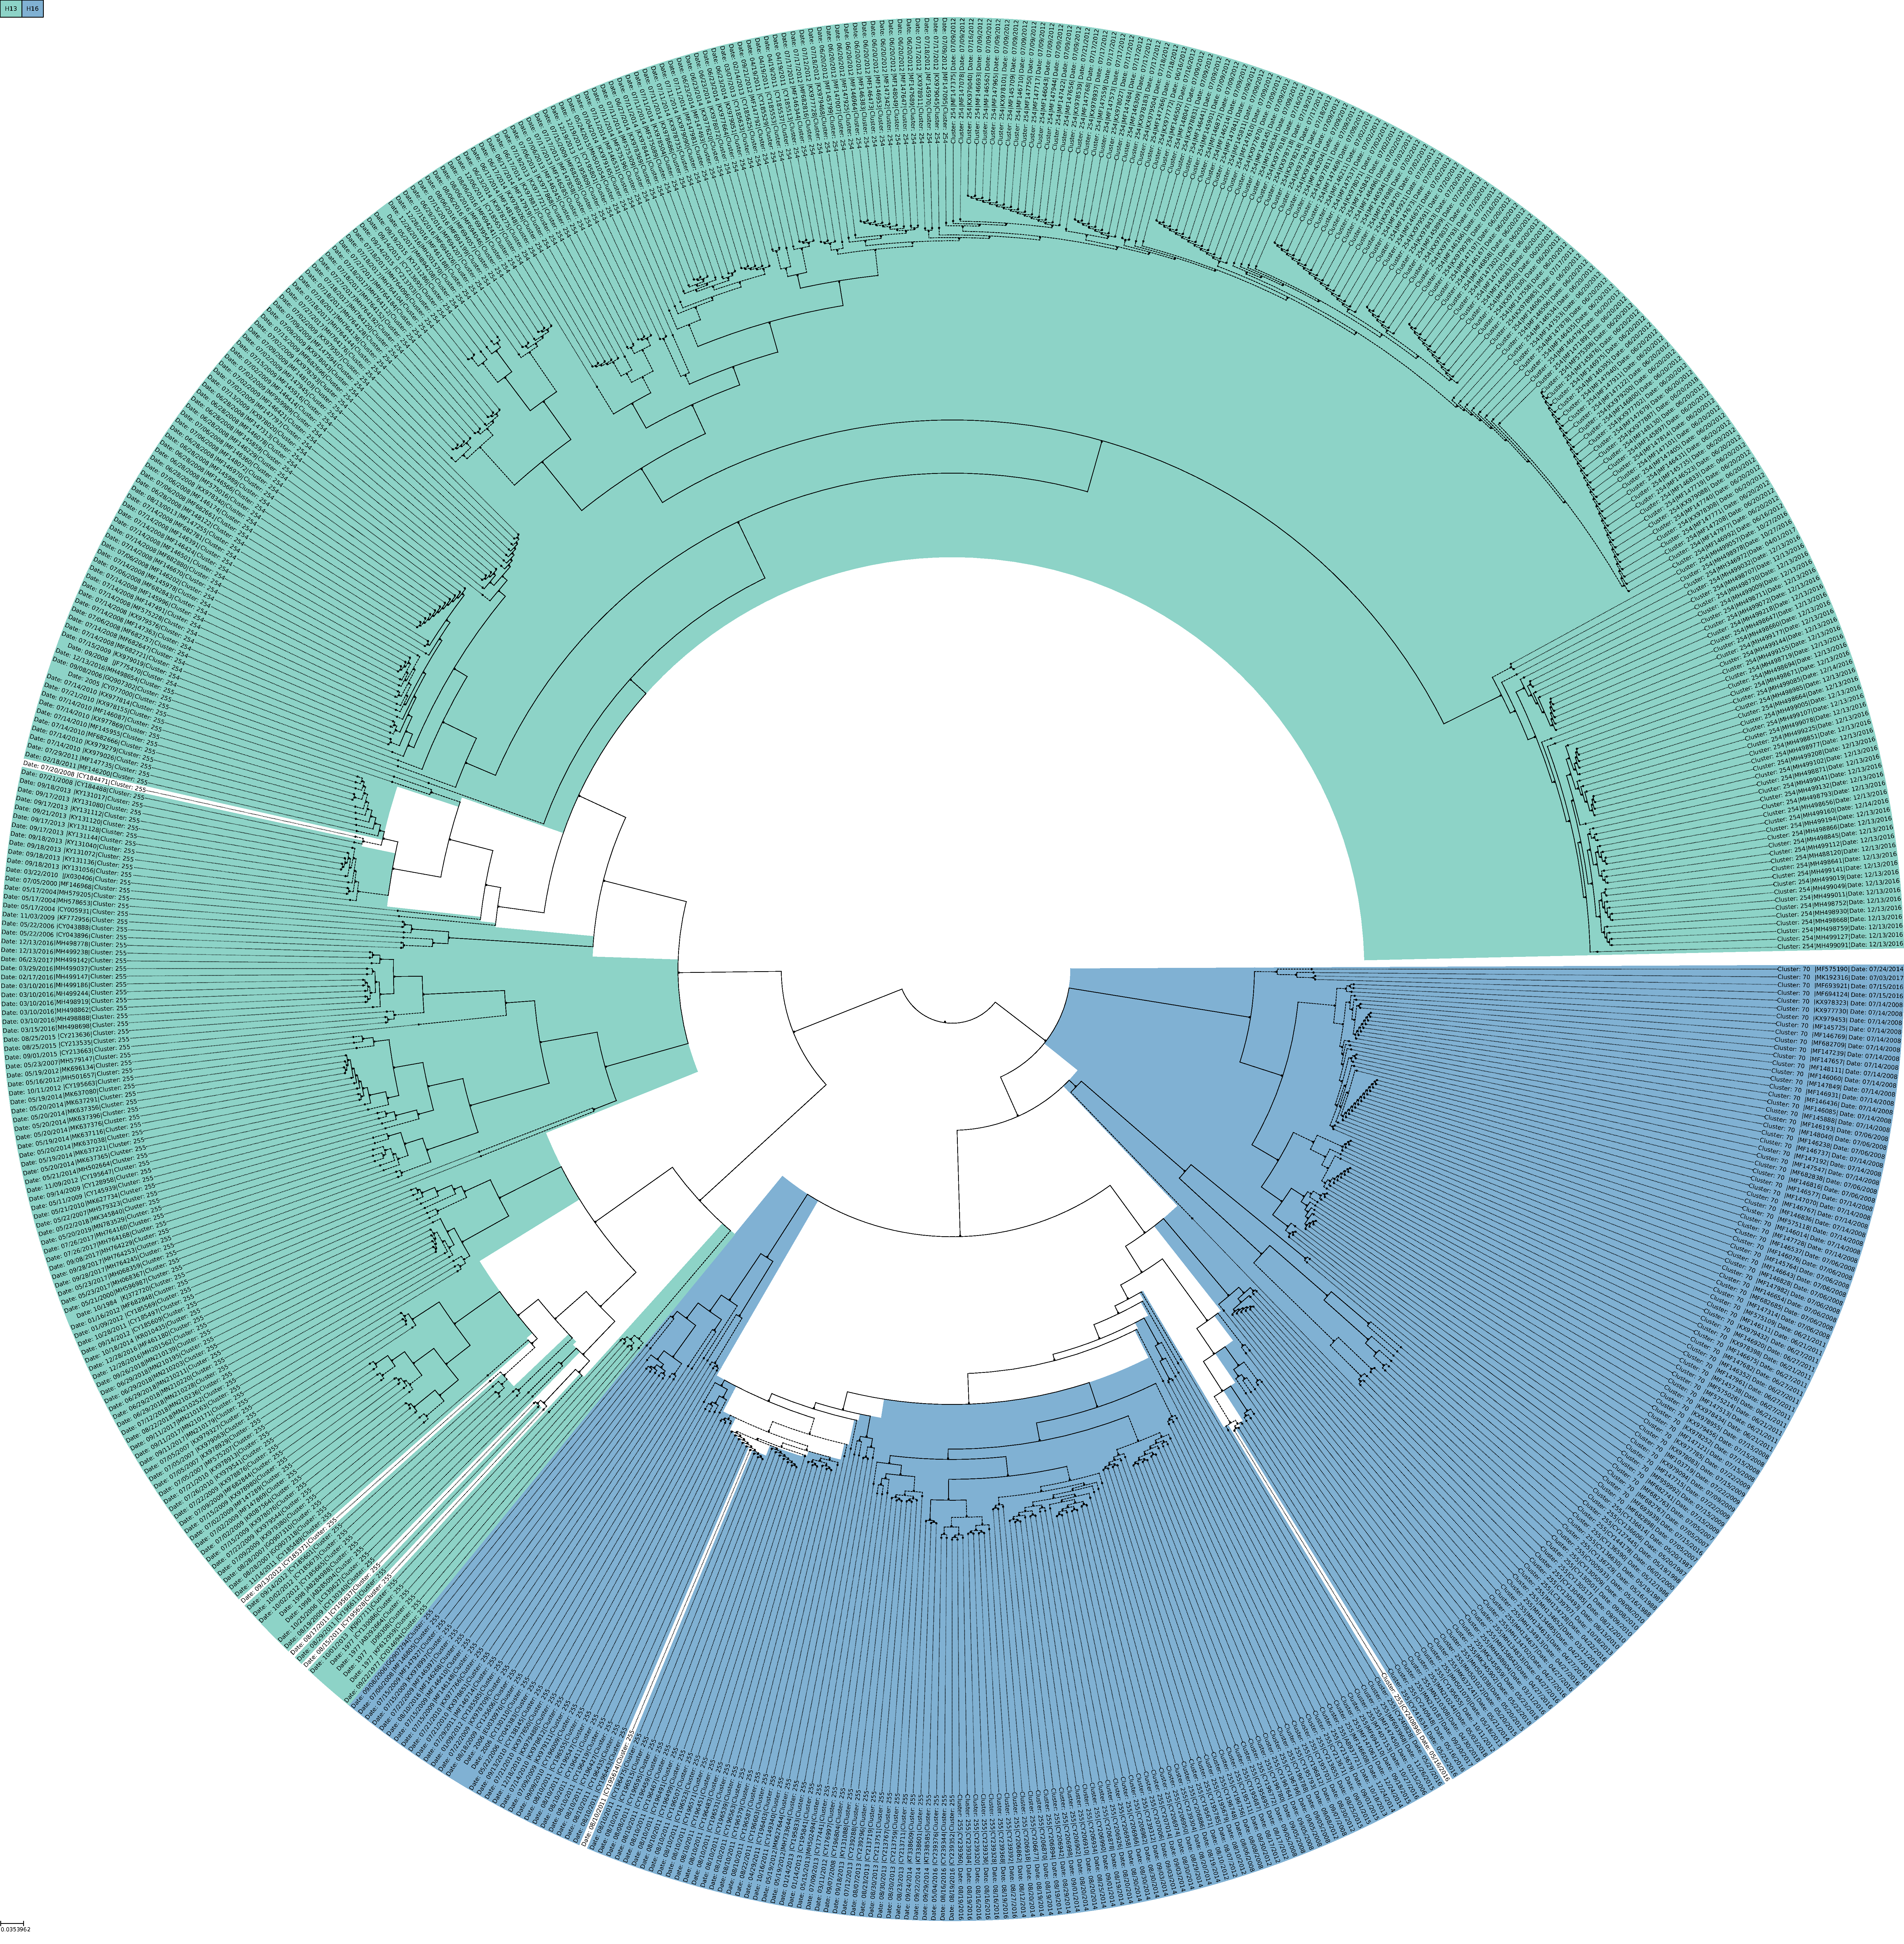
\includegraphics[width=\textwidth]{UMAP/Precalculated_Segment_4_H_Cosine.pdf}
    \caption[H13/H16 Precalculated \Acrshort{UPGMA} Tree (cosine)]{\textbf{H13/H16 Precalculated \Acrshort{UPGMA} Tree (cosine).} .}
    \label{fig:Precalculated_Cosine}
\end{figure}

\begin{figure}[!hbt]
    \centering
    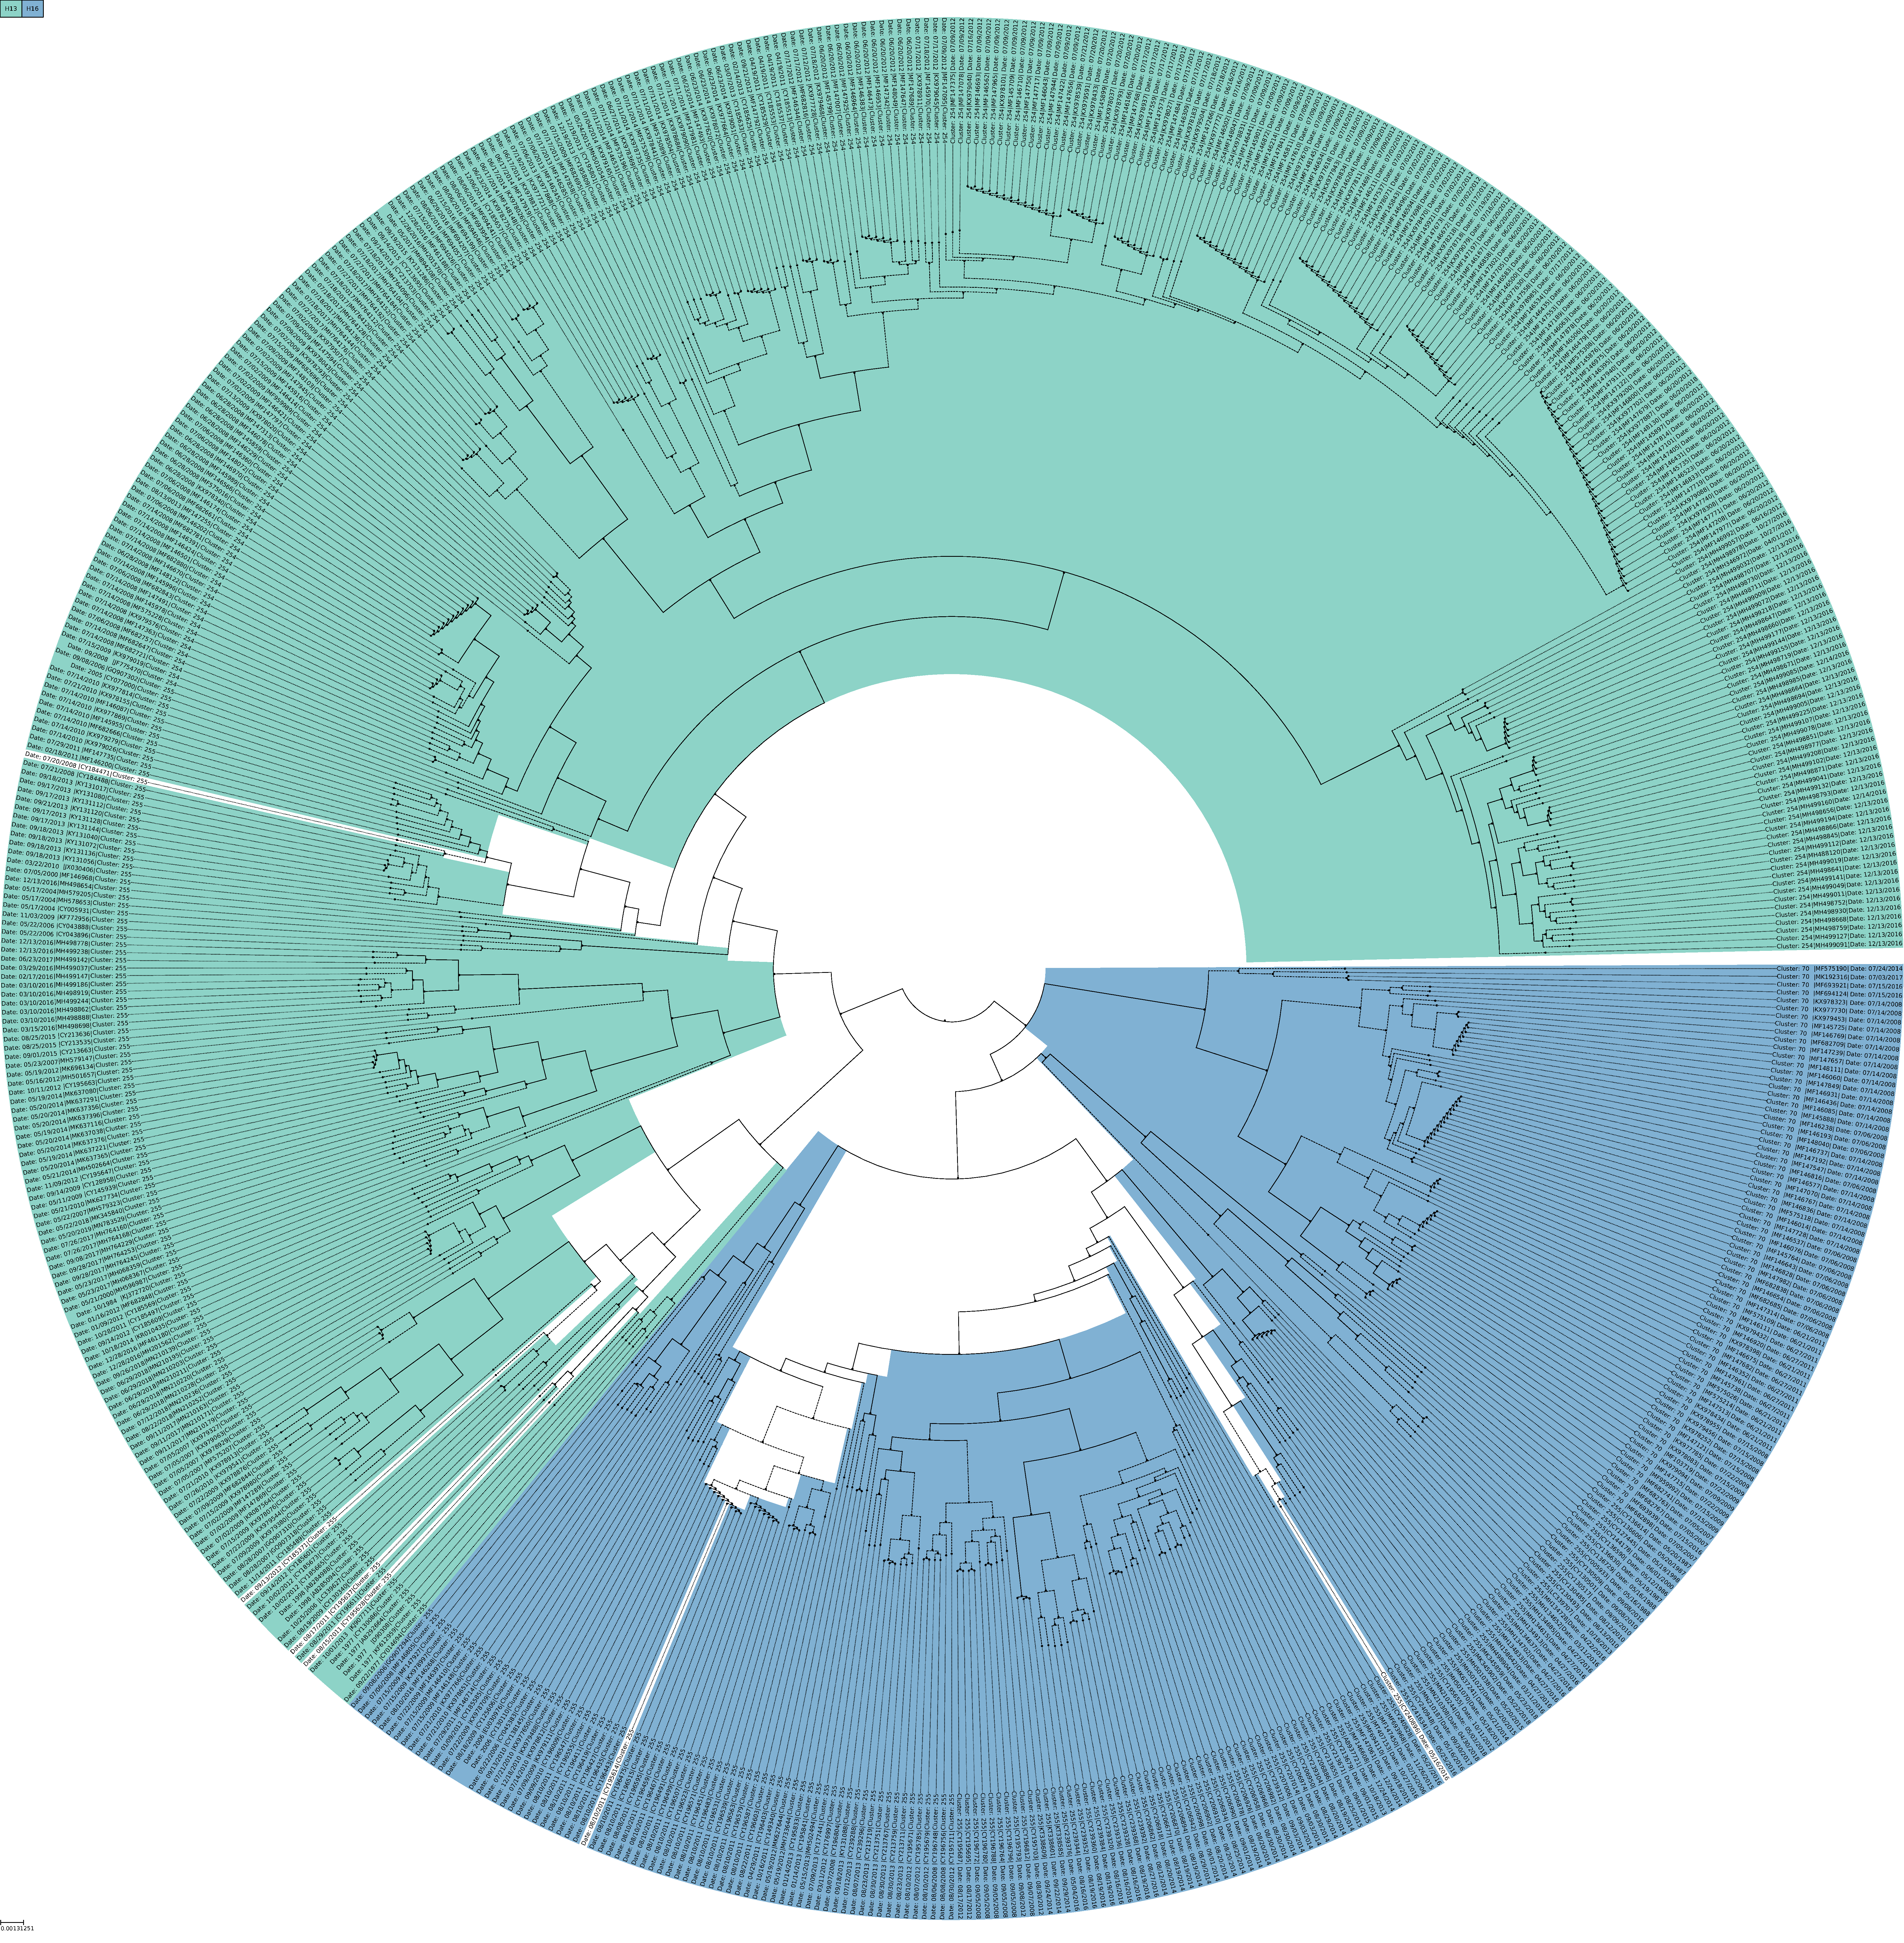
\includegraphics[width=\textwidth]{UMAP/Precalculated_Segment_4_H_Euclidean.pdf}
    \caption[H13/H16 Precalculated \Acrshort{UPGMA} Tree (euclidean)]{\textbf{H13/H16 Precalculated \Acrshort{UPGMA} Tree (euclidean).} .}
    \label{fig:Precalculated_Euclid}
\end{figure}

%frage is hier welche Methode die bessere representation ausstrahlt, sprich UMAP vgl. precalc ja/nein? dann PCA vgl precalc passt? ja/nein?